\chapter{Regular Languages}

\section{Finite Automata}

\begin{defination}
    A \textbf{finite automation} is a 5-tuple ($Q, \sum, \delta, q_0, F$) where

    \begin{enumerate}
        \item $Q$ is a finite set called the \textbf{states}
        \item $\sum$ is a finite set called the \textbf{alphabet}
        \item $\delta: Q \times \sum \rightarrow Q$ is the \textbf{transition
            function}
        \item $q_0 \in Q$ is the \textbf{start state}, and
        \item $F \subseteq Q$ is the \textbf{set of accept states}
    \end{enumerate}
\end{defination}

If $A$ is the set of all strings that machine $M$ accepts, we say that $A$ is
the \textbf{language of machine $M$} and write $L(M) = A$. We say that
\textbf{$M$ recognizes $A$} or that \textbf{$M$ accepts $A$}.

A machine may accept several strings, but it always recognizes only one
lnaguage.

\subsubsection{Formal defination of Computation}

Let $M = (Q, \sum, \delta, q_0, F)$ be a finite automaton and let 
$w = w_1w_2\dots w_n$ be a string where each $w_i$ is a member of the alphabet
$\sum$. Then $M$ \textbf{accepts} w if a sequence of states $r_0, r_1, \dots,
r_n$ in $Q$ exists with three conditions:

\begin{enumerate}
    \item $r_0 = q_0$,
    \item $\delta(r_i, w_{i+1}) = r_{i+1}$, for $i = 0, \dots, n - 1$, and
    \item $r_n \in F$.
\end{enumerate}

Condition 1 says that the machine starts in the start state, Condition 2
says that the machine goes from the state to state according to the transition
function. Condtion 3 sayas that machine accepts its input if it ends up in
accept state. We say that $M$ \textbf{recognizes language} $A$ if
$A = \{w \mid M accepts w\}$

\begin{defination}
    A language is called a \textbf{regular language} if some finite automaton
    recognizes it.
\end{defination}

\subsection{The Regular Operations}

\begin{defination}
    Let $A$ and $B$ be languages. We define the regular operations
    \textbf{union, concatenation,} and \textbf{star} as follows:
    \begin{itemize}
        \item \textbf{Union} $A \cup B = \{x \mid x \in
            A\ \text{or}\ x \in B\}$.
        \item \textbf{Concatenation:} $A \circ B = \{xy \mid x \in
            A\ \text{and}\ y \in B\}$.
        \item $A^{*} = \{x_1x_2\dots x_k \mid k \ge 0\ \text{and each}\ x_i
            \in A\}$.
    \end{itemize}
\end{defination}

\section{NonDeterminism}

When the machine was in a given state and read the next input symbol, we knew
what the next state would be, it is determined. We call this
\textbf{deterministic} computation. In a \textbf{nondeterministic} machine,
several choices may exist for the next state at any point. Nondeterminism is
a generalization of determinism, so every deterministic finite automaton is
automatically a nondeterministic finite automaton.

\subsection{Formal defination of a nondeterministic finite automaton}

\begin{defination}
    A \textbf{nondeterministic finite automaton} is a 5-tuple
    $(Q, \sum, \delta, q_0, F)$, where
    \begin{enumerate}
        \item $Q$ is a finite set of states,
        \item $\sum$ is a finite alphabet,
        \item $\delta: Q \times \sum_{\epsilon} \rightarrow P(Q)$ is the 
            transition function,
        \item $q_0 \in Q$ is the start state, and
        \item $F \subseteq Q$ is the set of accept states.
    \end{enumerate}
\end{defination}

The formal defination of computation for an NFA is similar to that or a DFA.
Let $N = \{Q, \sum, \delta, q_0, F\}$ be an NFA and $w$ a string over the 
alphabet $\sum$. Then we say that $N$ \textbf{accepts} $w$ if we can write
$w$ as $w = y_1y_2\dots y_m$, where each $y_i$ is a member of $\sum_{\epsilon}$
and a sequence of states $r_0, r_1, \dots, r_m$ exists in $Q$ with three
conditions
\begin{enumerate}
    \item $r_0 = q_0$,
    \item $r_{i+1} \in \delta(r_i, y_{i+1})$, for $i = 0, \dots, m - 1$, and
    \item $r_m \in F$.
\end{enumerate}

Condition 1 says that the machine starts out in the start state. Condition 2
says that state $r_{i+1}$ is one of the allowable next states when $N$ is
in the state $r_i$ and reading $y_{i+1}$. Observe that $\delta(r_i, y_{i+1})$
is the \textit{set} of allowable next states and so we say that $r_{i+1}$
is a member of that set. Finally, condition 3 says that the machine accepts
its input if the last state is an accept state.

\subsection{Equivalence of NFAs and DFAs}

\begin{theorem}
    Every nondeterministic finite automaton has an equivalent deterministic
    finite automaton
\end{theorem}

\paragraph{Proof idea:} We keep track of of the current states and create
a transition function based on that. If there are $k$ states o the NFA, then
it has $2^{k}$ subsets of states. To keep track of these states, the DFA will
have $2^{k}$ states.

\begin{corollary}
    A language is regular if and only if some nondeterministic finite automaton
    recognizes it.
    \label{140}
\end{corollary}

\subsection{Closure under the regular operations}

\begin{theorem}
    The class of regular languages is closed under the union operation
\end{theorem}

\textbf{Proof:} Let:

\begin{align*}
    N_1 &= (Q_1, \sum, \delta_1, q_1, F_1) \text{recognize $A_1$, and}\\
    N_2 &= (Q_2, \sum, \delta_2, q_2, F_2) \text{recognize $A_2$.}
\end{align*}

Construct $N = (Q, \sum, \delta, q_0, F)$ to recognize $A_1 \cup A_2$.

\begin{enumerate}
    \item $Q = \{q_0\} \cup Q_1 \cup Q_2$\\
        The states of $N$ are all the states of $N_1$ and $N_2$, with the
        addition of a new start state $q_0$.
    \item The state $q_0$ is the start state of $N$.
    \item The set of accept states $F = F_1 \cup F_2$.
    \item Define $\delta$ so that for any $q \in Q$ and any $a \in
        \sum_{\epsilon}$,

        $$
            \delta(q, a) = 
            \begin{cases}
                \delta_1(q, a) & q \in Q_1\\
                \delta_2(q, a) & q \in Q_2\\
                \{q_1, q_2\} & q = q_0 \text{and} a = \epsilon\\
                \phi & q = q_0 \text{and} a \neq \epsilon
            \end{cases}
        $$
\end{enumerate}

\begin{figure}[h!]
    \begin{center}
        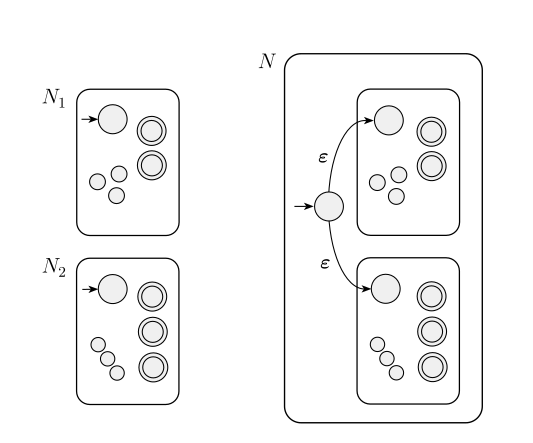
\includegraphics[width=5cm]{img/146.png}
        \caption{Construction of an NFA $N$ to recognize $A_1 \cup A_2$}
    \end{center}
\end{figure}

\begin{theorem}
    The class of regular languages is closed under the concatenation operation
\end{theorem}

The formal proof is similar to the previous proof. The follwing image describes
the contruction:

\begin{figure}[h!]
    \begin{center}
        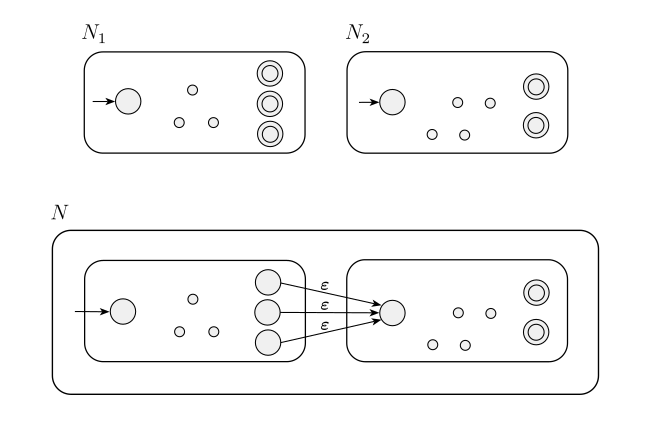
\includegraphics[width=5cm]{img/148.png}
        \caption{Construction of $N$ to recognize $A_1 \circ A_2$}
    \end{center}
\end{figure}

\begin{theorem}
    The class of regular languages is closed under the star operation.
\end{theorem}

The formal proof is similar to union proof. The following image describes the
construction:

\begin{figure}[h!]
    \begin{center}
        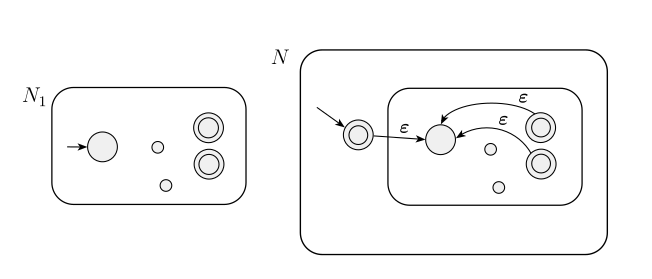
\includegraphics[width=5cm]{img/150.png}
        \caption{Construction of $N$ to recognize $A^{*}$}
    \end{center}
\end{figure}

\section{Regular Expressions}

In arthimetic, we can use operations $+$ and $\times$ to build up expressions
such as 

$$
(5 + 3) \times 4
$$

Similarly, we can use the regular operations to build up expressions describing
languages, which are called \textbf{regular expressions}. Example:

$$
(0 \cup 1)0^{*}
$$

\begin{defination}
    Say that $R$ is a \textbf{regular expression} if R is
    \begin{enumerate}
        \item $a$ for some $a$ in the alphabet $\sum$,
        \item $\epsilon$,
        \item $\phi$,
        \item $(R_1 \cup R_2)$, where $R_1$ and $R_2$ are regular expressions,
        \item $(R_1 \circ R_2)$, where $R_1$ and $R_2$ are regular
            expressions, or
        \item $(R_1^{*})$, were $R_1$ is a regular expression.
    \end{enumerate}
\end{defination}

\subsection{Equivalence with finite automata}

\begin{theorem}
    A language is regular if and only if some regular expression describes it.
\end{theorem}

This theorem has two directions that we will prove.

\begin{lemma}
    If a language is described by a regular expression, then it is regular.
\end{lemma}

\textbf{Proof Idea:} We can show how to convert $R$ into an NFA recognizing $A$
. By Corolary \ref{140}, if an NFA recofnizes $A$ then $A$ is regular. This
can be done by proving that for each of the 6 cases of regular expressions, 
we can build a NFA for it.

\begin{lemma}
    If a language is regular, then it is described by a regular expression.
\end{lemma}

\textbf{Proof:} We need to show that if a language $A$ is regular, a regular
expression describes it. Because $A$ is regular, it is accepted by a DFA. We
describe a procedure for converting DFAs into equivalent regular expressions.\\

We will first define a new type of finite automaton called a
\textbf{generalized nondeterministic finite automaton}, GNFA. First we show
how to convert DFAs into GNFAs, and then GNFAs into regular expressions.\\

GNFA are simply NDA wherein the transition arrows may have any regular
expression as labels, instead of only members of the alphabet or $\epsilon$.

\begin{figure}[h!]
    \begin{center}
        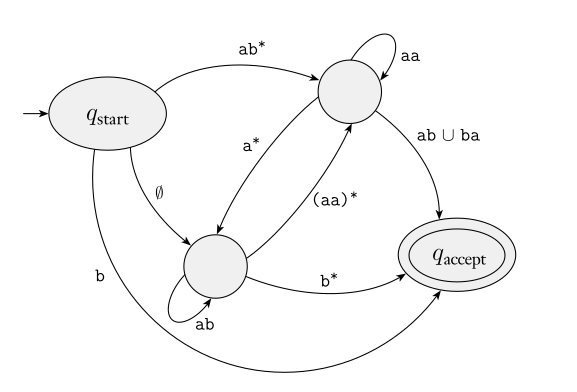
\includegraphics[width=5cm]{img/161.png}
        \caption{A generalized nondeterministic finite automaton}
    \end{center}
\end{figure}

For convenience, we require that GNFAs always have a special form that meets
the following conditions.

\begin{itemize}
    \item The start state has transition arrows going to every other state but
        no arrows coming in from any other state.
    \item There is only a single accept state, and it has arrows coming in
        from every other state but no arrows going to any other state. 
        Furthermore, the accept state is not the same at the start state.
    \item Except for the start and accept states, one arrow goes from the
        every state to every other state and also from each state to itself.
\end{itemize}

It is easy to convert a DFA into a GNFA in the special form. We simply add a
new start state with an $\epsilon$ to the old start state and a new accept
state with $\epsilon$ arrows from the old accept states. If any arrows have
multiple labes, we take union of the previous labels. Finally, we add arrows
labeled $\phi$ between states that had no arrows.\\

To convert GNFA into a regular expression, we take a $k$ state GNFA, and form 
an equivalent $k - 1$ state GNFA. If $k = 2$, The GNFA has a single arrow
from accept state to the end state, the label of which is the required 
regular expression.\\

To construct a GNFA with one fewer state, we do this:

\begin{figure}[h!]
    \begin{center}
        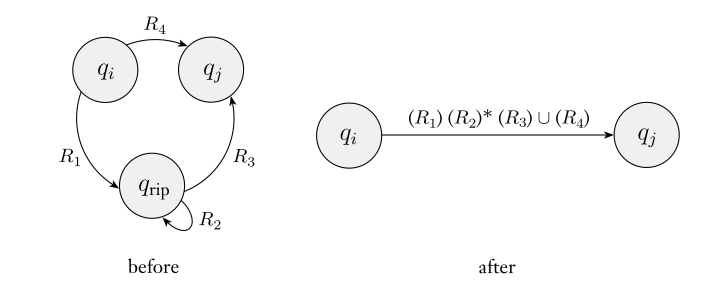
\includegraphics[width=5cm]{img/163.png}
        \caption{Constructing an equivalent GNFA with one fewer state}
    \end{center}
\end{figure}

We do this for every pair $q_i. q_j$.

Formal Defination:

\begin{defination}
    A \textbf{generalized nondeterministic finite automaton} is a 5-tuple,
    $(Q, \sum, \delta, q_{start}, q_{accept})$, where
    \begin{enumerate}
        \item $Q$ is the finite set of states,
        \item $\sum$ is the input alphabet,
        \item $\delta: (Q - \{q_{accept}\}) \times (Q - \{q_{start}\}) 
            \rightarrow R$ is the transition function,
        \item $q_{start}$ is the start state, and
        \item $q_{accept}$ is the accept state.
    \end{enumerate}
\end{defination}

\section{Non-Regular Languages}

